\documentclass[11pt]{article}
\usepackage[utf8]{inputenc}
\usepackage[T1]{fontenc}
\usepackage{amsmath}
\usepackage{amssymb}
\usepackage{multicol}
\usepackage{geometry}
\usepackage{tikz}
\usetikzlibrary{shapes,patterns,angles,quotes}
\usepackage{enumitem}
\usepackage{xcolor}
\usepackage{titlesec}

% Configurações de layout
\geometry{a4paper, left=1cm, right=1cm, top=0.5cm, bottom=1.2cm}
\setlength{\columnseprule}{0.4pt}

% Cores para títulos
\titleformat{\section}{\normalfont\Large\bfseries\color{blue}}{\thesection}{1em}{}
\titleformat{\subsection}{\normalfont\large\bfseries\color{red}}{\thesubsection}{1em}{}

\title{\textcolor{blue}{Geometria Plana
    \\Polígonos: Elementos e Propriedades}}
\author{Professor: Jefferson}
\date{}

\begin{document}

\maketitle
\vspace{-1cm}

%\begin{center}
%\large{Nome: \underline{\hspace{8cm}} \quad Turma: \underline{\hspace{3cm}}}
%\end{center}

\begin{multicols}{2}

\section*{Elementos de um Polígono}

\begin{center}
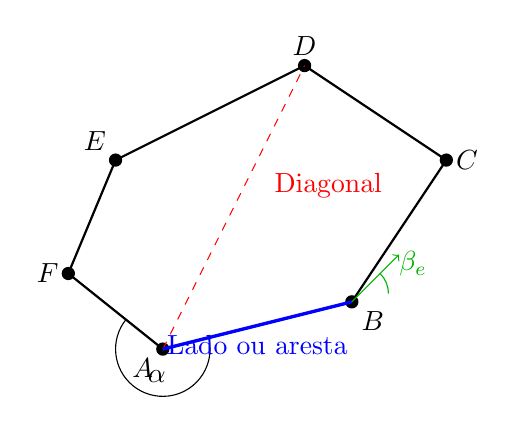
\begin{tikzpicture}[scale=1.2]
% Polígono irregular
\coordinate (A) at (0,0);
\coordinate (B) at (2,0.5);
\coordinate (C) at (3,2);
\coordinate (D) at (1.5,3);
\coordinate (E) at (-0.5,2);
\coordinate (F) at (-1,0.8);

% Desenhar polígono
\draw[thick] (A) -- (B) -- (C) -- (D) -- (E) -- (F) -- cycle;

% Vértices
\foreach \point/\position in {A/below left, B/below right, C/right, D/above, E/above left, F/left} {
    \fill (\point) circle (2pt);
    \node[\position] at (\point) {$\point$};
}

% Ângulo interno em A
\draw pic[draw, angle radius=6mm, "$\alpha$"] {angle = F--A--B};

% Diagonal
\draw[red, dashed] (A) -- (D);
\node[red, above] at (1.75,1.5) {Diagonal};

% Lado AB
\draw[blue, very thick] (A) -- (B);
\node[blue, below] at (1,0.25) {Lado ou aresta};

% Ângulo externo
\draw[->, green!70!black] (2,0.5) -- (2.5,1);
\draw[green!70!black] (2.3,0.8) arc (45:0:0.3);
\node[green!70!black, right] at (2.4,0.9) {$\beta_e$};
\end{tikzpicture}
\end{center}

\subsection*{Definições}
\begin{itemize}
\item \textbf{Vértice}: Ponto de encontro de dois lados ($A, B, C, \dots$)
\item \textbf{Lado/Aresta}: Segmento que une dois vértices consecutivos
\item \textbf{Ângulo interno}: Ângulo formado por dois lados consecutivos ($\alpha$)
\item \textbf{Ângulo externo}: Ângulo formado por um lado e o prolongamento do lado adjacente ($\beta_e$)
\item \textbf{Diagonal}: Segmento que une dois vértices não consecutivos
\end{itemize}

\section*{Classificação dos Polígonos}

\subsection*{Quanto ao número de lados}

\begin{center}
\begin{tabular}{|c|c|c|}
\hline
\textbf{Nº de lados} & \textbf{Nome} & \textbf{Figura} \\
\hline
3 & Triângulo & △ \\
4 & Quadrilátero & □ \\
5 & Pentágono & ⬠ \\
6 & Hexágono & ⬡ \\
7 & Heptágono & \\
8 & Octógono & ⬢ \\
9 & Eneágono & \\
10 & Decágono & \\
\hline
\end{tabular}
\end{center}

\subsection*{Quanto à regularidade}
\begin{itemize}
\item \textbf{Regular}: Todos os lados e ângulos iguais
\item \textbf{Irregular}: Lados ou ângulos diferentes
\end{itemize}

\subsection*{Quanto à forma}
\begin{itemize}
\item \textbf{Convexo}: Todas as diagonais estão no interior
\item \textbf{Côncavo}: Alguma diagonal está no exterior
\end{itemize}

\section*{Fórmulas Fundamentais}

\subsection*{Soma dos Ângulos Internos}

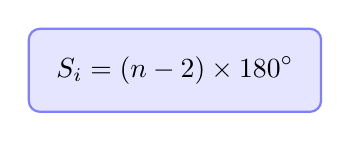
\begin{tikzpicture}
\node[rectangle, fill=blue!10, rounded corners, inner sep=10pt, draw=blue!50, thick] (box) {
$\displaystyle S_i = (n - 2) \times 180^\circ$
};
\end{tikzpicture}

\textbf{Onde:}
\begin{itemize}
\item $S_i$ = soma dos ângulos internos
\item $n$ = número de lados (vértices)
\end{itemize}

\textbf{Exemplos:}
\begin{itemize}
\item Triângulo $(n=3)$: $S_i = 180^\circ$
\item Quadrilátero $(n=4)$: $S_i = 360^\circ$
\item Pentágono $(n=5)$: $S_i = 540^\circ$
\end{itemize}

\subsection*{Soma dos Ângulos Externos}

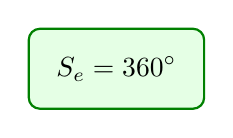
\begin{tikzpicture}
\node[rectangle, fill=green!10, rounded corners, inner sep=10pt, draw=green!50!black, thick] (box) {
$\displaystyle S_e = 360^\circ$
};
\end{tikzpicture}

\textbf{Importante:} A soma dos ângulos externos de qualquer polígono convexo é sempre $360^\circ$, independente do número de lados.

\subsection*{Número de Diagonais}

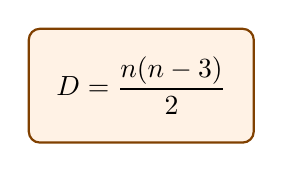
\begin{tikzpicture}
\node[rectangle, fill=orange!10, rounded corners, inner sep=10pt, draw=orange!50!black, thick] (box) {
$\displaystyle D = \frac{n(n-3)}{2}$
};
\end{tikzpicture}

\textbf{Onde:}
\begin{itemize}
\item $D$ = número total de diagonais
\item $n$ = número de lados
\end{itemize}

\textbf{Exemplos:}
\begin{itemize}
\item Quadrilátero $(n=4)$: $D = 2$
\item Pentágono $(n=5)$: $D = 5$
\item Hexágono $(n=6)$: $D = 9$
\end{itemize}

\subsection*{Ângulo Interno de Polígono Regular}

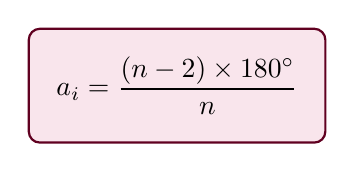
\begin{tikzpicture}
\node[rectangle, fill=purple!10, rounded corners, inner sep=10pt, draw=purple!50!black, thick] (box) {
$\displaystyle a_i = \frac{(n-2) \times 180^\circ}{n}$
};
\end{tikzpicture}

\textbf{Onde:}
\begin{itemize}
\item $a_i$ = medida de cada ângulo interno
\item $n$ = número de lados
\end{itemize}

\subsection*{Ângulo Externo de Polígono Regular}

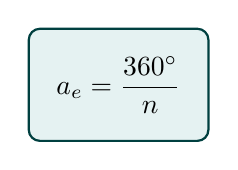
\begin{tikzpicture}
\node[rectangle, fill=teal!10, rounded corners, inner sep=10pt, draw=teal!50!black, thick] (box) {
$\displaystyle a_e = \frac{360^\circ}{n}$
};
\end{tikzpicture}

\section*{Relações Importantes}

\subsection*{Relação entre Ângulos}
Para qualquer polígono:
\[
a_i + a_e = 180^\circ
\]

\subsection*{Número de Triângulos}
Um polígono de $n$ lados pode ser dividido em $(n-2)$ triângulos traçando diagonais a partir de um vértice.

\subsection*{Fórmula de Euler (para poliedros)}
Para polígonos no plano:
\[
V - A + F = 1
\]
\textbf{Onde:}
\begin{itemize}
\item $V$ = número de vértices
\item $A$ = número de arestas
\item $F$ = número de faces (1 para polígono plano)
\end{itemize}

\section*{Exercícios de Fixação}

\begin{enumerate}[leftmargin=*]

\item Complete a tabela:

\begin{center}
\begin{tabular}{|c|c|c|c|c|}
\hline
\textbf{Polígono} & \textbf{n} & \textbf{$S_i$} & \textbf{$a_i$ (regular)} & \textbf{Diagonais} \\
\hline
Triângulo & 3 & & $60^\circ$ & 0 \\
\hline
Quadrilátero & 4 & $360^\circ$ & & 2 \\
\hline
Pentágono & 5 & & $108^\circ$ & \\
\hline
Hexágono & 6 & & & 9 \\
\hline
Heptágono & 7 & $900^\circ$ & & \\
\hline
Octógono & 8 & & $135^\circ$ & \\
\hline
\end{tabular}
\end{center}

\item Calcule para um polígono com:
\begin{enumerate}[label=\alph*)]
\item 12 lados: a soma dos ângulos internos
\item 15 lados: o número total de diagonais
\item 20 lados: o ângulo interno se for regular
\end{enumerate}

\item Dado que a soma dos ângulos internos de um polígono é $1440^\circ$:
\begin{enumerate}[label=\alph*)]
\item Quantos lados tem o polígono?
\item Quantas diagonais possui?
\item Qual o ângulo externo se for regular?
\end{enumerate}

\item Um polígono regular tem ângulo interno de $150^\circ$:
\begin{enumerate}[label=\alph*)]
\item Quantos lados tem?
\item Calcule o ângulo externo
\item Quantas diagonais possui?
\end{enumerate}

\item Para um hexágono regular:
\begin{center}
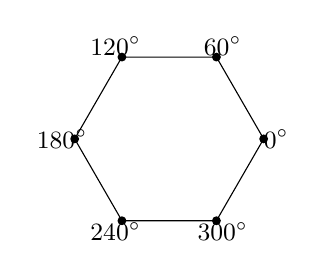
\begin{tikzpicture}[scale=0.8]
\draw (0:1.5) -- (60:1.5) -- (120:1.5) -- (180:1.5) -- (240:1.5) -- (300:1.5) -- cycle;
\foreach \angle in {0,60,120,180,240,300} {
    \fill (\angle:1.5) circle (2pt);
    \node at (\angle:1.7) [font=\small] {$\angle^\circ$};
}
\end{tikzpicture}
\end{center}
\begin{enumerate}[label=\alph*)]
\item Calcule a soma dos ângulos internos
\item Calcule a medida de cada ângulo interno
\item Calcule o número de diagonais
\item Trace todas as diagonais a partir de um vértice
\end{enumerate}

\item Problema de vértices e arestas:
\begin{enumerate}[label=\alph*)]
\item Um polígono tem 9 vértices. Quantas arestas tem?
\item Se um polígono tem 14 arestas, quantos vértices tem?
\item Verifique a relação $V = A$ para polígonos
\end{enumerate}

\item Ângulos internos e externos:
\begin{enumerate}[label=\alph*)]
\item Em um polígono regular, $a_i = 5 \times a_e$. Quantos lados tem?
\item Se $a_i - a_e = 100^\circ$ em um polígono regular, encontre $n$
\end{enumerate}

\item Diagonais por vértice:
\begin{enumerate}[label=\alph*)]
\item De um único vértice de um polígono de $n$ lados, quantas diagonais podem ser traçadas?
\item Prove que: diagonais por vértice = $n - 3$
\end{enumerate}

\item Polígono convexo vs côncavo:
\begin{center}
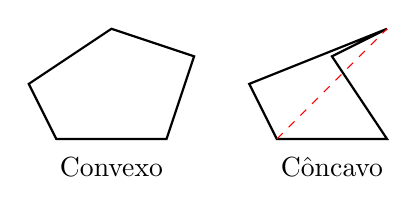
\begin{tikzpicture}[scale=0.7]
% Convexo
\begin{scope}
\draw[thick] (0,0) -- (2,0) -- (2.5,1.5) -- (1,2) -- (-0.5,1) -- cycle;
\node at (1, -0.5) {Convexo};
\end{scope}
% Côncavo
\begin{scope}[xshift=4cm]
\draw[thick] (0,0) -- (2,0) -- (1,1.5) -- (2,2) -- (-0.5,1) -- cycle;
\node at (1, -0.5) {Côncavo};
\draw[red, dashed] (0,0) -- (2,2);
\end{scope}
\end{tikzpicture}
\end{center}
\begin{enumerate}[label=\alph*)]
\item As fórmulas de soma de ângulos valem para ambos?
\item A fórmula do número de diagonais vale para ambos?
\end{enumerate}

\item Aplicação das fórmulas:
\begin{enumerate}[label=\alph*)]
\item Um polígono tem 35 diagonais. Quantos lados tem?
\item A soma dos ângulos internos de um polígono é o quádruplo da soma dos ângulos externos. Quantos lados tem?
\end{enumerate}

\end{enumerate}

\section*{Problemas Avançados}

\begin{enumerate}[leftmargin=*, start=11]

\item Relação entre lados e diagonais:
\begin{enumerate}[label=\alph*)]
\item Prove que em um polígono convexo de $n$ lados:
  \[
  \text{Nº de diagonais} = \frac{n(n-3)}{2}
  \]
\item Use indução matemática para provar a fórmula
\end{enumerate}

\item Polígono estrelado:
\begin{center}
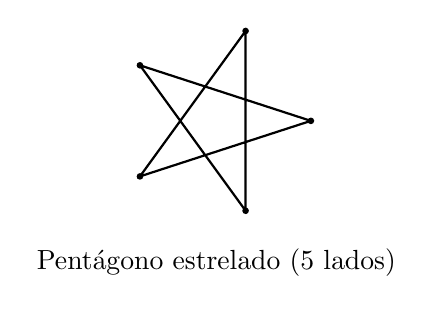
\begin{tikzpicture}[scale=0.6]
\draw[thick] (0:2) -- (144:2) -- (288:2) -- (72:2) -- (216:2) -- cycle;
\foreach \angle in {0,72,144,216,288} {
    \fill (\angle:2) circle (2pt);
}
\node at (0, -3) {Pentágono estrelado (5 lados)};
\end{tikzpicture}
\end{center}
\begin{enumerate}[label=\alph*)]
\item Quantas arestas tem um pentágono estrelado?
\item As fórmulas estudadas se aplicam?
\end{enumerate}

\item Generalização para polígonos côncavos:
\begin{enumerate}[label=\alph*)]
\item A fórmula $S_i = (n-2) \times 180^\circ$ vale para polígonos côncavos?
\item E a fórmula das diagonais?
\end{enumerate}

\item Polígono com diagonais que não se cruzam:
\begin{enumerate}[label=\alph*)]
\item Para $n=4$, temos 2 diagonais que se cruzam
\item Para $n=5$, temos 5 diagonais. Quantos cruzamentos?
\item Encontre uma fórmula para o número máximo de cruzamentos de diagonais
\end{enumerate}

\item Relação com combinações:
\begin{enumerate}[label=\alph*)]
\item Mostre que o número de diagonais é $C_n^2 - n$
\item Justifique geometricamente
\end{enumerate}

\item Ângulos em vértices consecutivos:
\begin{enumerate}[label=\alph*)]
\item Em um polígono regular de $n$ lados, qual a medida do ângulo central?
\item Mostre que o ângulo central = ângulo externo
\end{enumerate}

\item Polígono inscrito em círculo:
\begin{center}
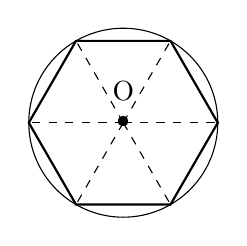
\begin{tikzpicture}[scale=0.8]
\draw (0,0) circle (1.5);
\draw[thick] (0:1.5) -- (60:1.5) -- (120:1.5) -- (180:1.5) -- (240:1.5) -- (300:1.5) -- cycle;
\foreach \angle in {0,60,...,300} {
    \draw[dashed] (0,0) -- (\angle:1.5);
}
\node at (0,0) {•};
\node[above] at (0,0.2) {O};
\end{tikzpicture}
\end{center}
\begin{enumerate}[label=\alph*)]
\item Qual a relação entre o ângulo central e o ângulo interno?
\item Para hexágono regular: ângulo central = $60^\circ$, $a_i = 120^\circ$
\end{enumerate}

\item Sequência de polígonos:
\begin{enumerate}[label=\alph*)]
\item Triângulo: $S_i = 180^\circ$, $D = 0$
\item Quadrilátero: $S_i = 360^\circ$, $D = 2$
\item Pentágono: $S_i = 540^\circ$, $D = 5$
\item Encontre o padrão e preveja para $n=10$
\end{enumerate}

\item Fórmula alternativa para $a_i$:
\begin{enumerate}[label=\alph*)]
\item Mostre que: $a_i = 180^\circ - \dfrac{360^\circ}{n}$
\item Deduza a partir das fórmulas conhecidas
\end{enumerate}

\item Desafio final:
\begin{enumerate}[label=\alph*)]
\item Um polígono tem o número de diagonais igual ao número de lados. Qual é este polígono?
\item Existe polígono cujo número de diagonais é o dobro do número de lados?
\end{enumerate}

\end{enumerate}

\section*{Resumo das Fórmulas}

\subsection*{Para qualquer polígono convexo de $n$ lados:}
\begin{itemize}
\item Número de vértices: $V = n$
\item Número de arestas: $A = n$
\item Soma dos ângulos internos: $S_i = (n-2) \times 180^\circ$
\item Soma dos ângulos externos: $S_e = 360^\circ$
\item Número de diagonais: $D = \dfrac{n(n-3)}{2}$
\end{itemize}

\subsection*{Para polígono regular de $n$ lados:}
\begin{itemize}
\item Ângulo interno: $a_i = \dfrac{(n-2) \times 180^\circ}{n}$
\item Ângulo externo: $a_e = \dfrac{360^\circ}{n}$
\item Relação: $a_i + a_e = 180^\circ$
\item Ângulo central: $a_c = \dfrac{360^\circ}{n} = a_e$
\end{itemize}

\subsection*{Relações derivadas:}
\begin{itemize}
\item De um vértice: $(n-3)$ diagonais
\item Formam $(n-2)$ triângulos
\item $D = C_n^2 - n$
\item $a_i = 180^\circ - a_e$
\end{itemize}

\section*{Dicas para Resolução}

\begin{itemize}
\item \textbf{Sempre identifique $n$}: Número de lados/vértices
\item \textbf{Use fórmulas adequadamente}: Verifique se polígono é regular
\item \textbf{Desenhe quando possível}: Ajuda na visualização
\item \textbf{Verifique unidades}: Ângulos em graus
\item \textbf{Faça testes}: Valores devem fazer sentido geometricamente
\end{itemize}

\section*{Aplicações Práticas}

\begin{itemize}
\item \textbf{Arquitetura}: Formas de construções
\item \textbf{Design}: Padrões geométricos
\item \textbf{Natureza}: Colmeias hexagonais
\item \textbf{Esportes}: Campos e quadras
\item \textbf{Tecnologia}: Pixels e displays
\end{itemize}

\end{multicols}

\end{document}
